%!TEX root = pfe-book4.tex
%!TEX TS-program = pdflatex
%!TEX encoding = UTF-8 Unicode


\cleardoublepage
%\mainmatter
\chapter[The Physics of the Universe]{The Physics of \\the Universe}
\label{ch-07}

\section{Measuring Distances to the Stars}

Today it is no longer possible to draw a strict boundary line between astronomy and physics. As long as astrono­mers, like geographers, confined themselves to descriptions of the stellar sky, the subject of astronomy drew small attention from physicists. However, the situation changed radically a few decades ago, particularly after observations began to be made from artificial earth satellites and the moon.

Without the terrestrial atmosphere as a hindrance, it is possible to receive all signals coming to us from the far corners of the universe. These include fluxes of a va­riety of particles and electromagnetic radiation of practi­cally the whole spectrum, from gamma rays to radio waves. And opportunities for observing the stars in the visible portion of the spectrum have increased immeasur­ably.

Now the study of particle fluxes and radiation of the electromagnetic spectrum most definitely belong in the sphere of physics. If we also note that studying outer space brings us face to face with a great diversity of phenomena that do not as yet bow to a unique interpre­tation and if we further note that we can and must be prepared for the physics of the universe leading to the discovery of entirely new laws of nature, it becomes clear why explorers of the stellar world are today mostly
physicists -- physicists by education and mode of thought.

We begin our discussion of the universe with a classical problem of astronomy. Measuring distances from the earth to distant stars. At the present time, the distances be­ tween the earth and the sun or the earth and the planets are measured to a high degree of accuracy by means of radar. The mean distance to the sun is equal to \num{149573000} kilometres. It has been calculated to within a millionth fraction of the distance.

\begin{figure}[!ht]
\centering
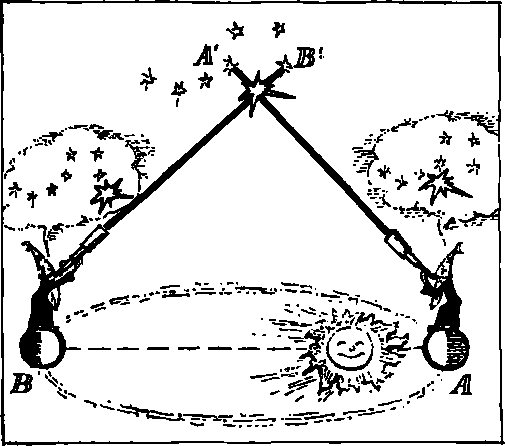
\includegraphics[width=0.8\textwidth]{figures/fig-07-01.pdf}
\caption{The parallax method to measure the distance to the stars.}
\label{fig-7.1}
\end{figure}

But astronomers had already measured distances inside the solar system without the aid of radar, using a simple (in principle) method called \emph{triangulation}.


Consider a group of stars, from two different spots, which should be as far apart as possible. This separation is termed the \emph{base} by astronomers. As sketched in \figr{fig-7.1}, astronomers first used very simple devices and, later, excellent telescopes to measure the angles between the directions to individual stars. They noticed that it is possible to choose a group of stars that moves across the sky as an integral whole. No matter what positions the stars are observed from, the angles between the directions to them remain the same. But among such stars they often found some one star that clearly moved with respect to its neighbours. Taking one of the ``fixed'' stars as a point of departure, it was possible to measure the angular displacement of the star that moved relative to the fixed constellation. That angle received the name \emph{parallax}.

As far back as the seventeenth century, after Galileo’s invention of the telescope, astronomers had already mea­sured the parallaxes of the planets by observing their displacements with respect to the ``fixed'' stars. It was then calculated that the earth is at a distance of 140 mil­lion kilometres from the sun. Very accurate indeed!

To the naked eye, the mutual positions of the stars remain unchanged. Only by taking photographs of the stars from different positions is it possible to detect parallactic displacements. The largest base for such a mea­surement is the diameter of the earth’s orbit. If we take two photographs of some portion of the sky from one and the same observatory with a time interval of half a year, the base will be equal to nearly 300 million kilometres.

Radar cannot be used to measure stellar distances and so the diagram shown in \figr{fig-7.1} is quite modern. 

This suggests that there are stars which are in perceptible motion relative to other stars. But it would be extremely illogical to assume that there are fixed stars and moving stars. The conclusion we are forced to is that the stars whose mutual positions remain unchanged are much farther away than a ``wandering'' star (or planet). Be that as it may, with good instruments we are in a position to measure the parallaxes of many stars.

Parallax measurements to within a hundredth of a second of arc have been carried out for many stars. It turned out that the stars closest to us lie at distances greater than one parsec.

A \emph{parsec} is the distance that yields an angular displacement of one second if the base is the diameter of the earth’s orbit. It is easy to calculate that one parsec is equal to 30 million million kilometres.

Astrophysicists also use what is known as the light year. The \emph{light year} is the distance traversed by light in one year. One parsec is equal to about 3.3 light years. Light travelling at \num{300000} kilometres a second takes half a day to cross the whole solar system. We now come to an important and amazing conclusion: our planetary system is very much alone in the universe.

The parallax method can be applied to distances of the order of hundreds of light years. We then have the prob­lem of how to measure distances to more distant stars. This turns out to be not at all simple, and any confidence in the correctness of approximate estimates (for the most part we can only be sure of one significant digit) is ob­tained by correlating results of different measurements.

At any rate, the decisive factor in determining dis­tances to faraway stars is that there are many so-called double stars among the millions upon millions of stars in our galaxy. Double stars also go by the name variable. The reason for this is clear: the brightness of the star varies because of the mutual motions of the two stars of the pair. The period of variation can be measured precise­ly.

Suppose we are observing a very distant cluster of stars. We are justified in concluding that the differences in observed brightness are not related to any difference in distance. We of course know about the inverse-square law (that is, the intensity of any radiation decreases with the inverse square of the distance), we also know about brightness diminishing if light rays pass through accumulations of stellar gas. But if a small patch of the night sky has been chosen and the stars are far away from us, they can be regarded as being in identical conditions.

Studies of double stars lying in the Small Magellanic Cloud led to the conclusion that there is a relationship between the period of a double star and its luminosity. This means that if certain stars are at approximately the same distance from us and the period of variation of brightness (this period is usually between 2 and 40 days) is the same, the stars will appear to be equally bright.

Having established this rule and being convinced of its usefulness, we can utilize it for stars that belong to different clusters. By comparing stars whose periods of variation are the same but whose brightnesses are different, we can assert that they lie at different distances from us. In order to determine how great these distances are, we can use the inverse-square law. But this method permits determining only the relative distances of variable stars from the earth. We can apply it only to very distant stars and cannot use it to calibrate our information about the absolute stellar-earth distances obtained in measuring parallactic displacements.

The scale for measuring distances between very distant stars was found by employing the Doppler effect.

The formulas that we discussed on page 187 of the third book of this series hold true for any vibrations. Therefore the frequencies of spectral lines observed in the spectrum of a star permit determining the velocity of the star away from the earth or towards the earth. Since in the equation
\begin{equation*}%
\nu' = \nu \left( 1 \pm \frac{v}{c} \right)
\end{equation*}
$c$ is the velocity of light (\SI{300000}{\kilo\meter\per\second}), it is clear that the star must have a high velocity and the spectrograph must be of extremely high quality for us to detect a dis­placement of the spectral lines.

Please note that the scientist is quite certain that the hydrogen on the star (that is, the hydrogen that has signalled to us) at an unimaginably colossal distance from us is the very same hydrogen that we deal with here on the earth. If the star were at rest, the hydrogen spectrum would have to be exactly like the spectrum we obtain from a gas-discharge tube (that is how confident the physicist is of the unity of the world!). But the lines are noticeably shifted and stellar velocities are in the hun­dreds and even tens of thousands of kilometres a second. No one has any doubts about this explanation. How could there be? The spectrum of hydrogen consists of a very large number of lines, and we see the displacement of all lines (not just one) of the spectrum in perfect accord with the Doppler equation.

But let us return to the measuring of stellar distances. Of what help can our knowledge of stellar velocities be? It is very simple. Provided of course that you have observed the star to have moved a certain distance during the year (all this of course with respect to other stars, which in this case may be regarded as ``fixed''). If we know the arc displacement $\varphi$ of a star ($\varphi$ being perpendic­ular to the light ray that reaches us), then, knowing the tangential velocity, we can find the distance to the star $R$ from the formula
\begin{equation*}%
\frac{R \varphi}{t} = v
\end{equation*}
In place of $t$ we can substitute the time of translation of the star.

But, says the reader, the formula involves the tangen­tial velocity, whereas we do not know the direction of motion of the star. Quite true, and that is why we have to take the following approach. A large number of double stars with the same blinking period are selected. Then the radial velocities of all these stars are measured. The radial velocity will vary from zero (if the star is moving at right angles to the ray of light) to a maximum (when the star is moving along the ray). If we assume that, on the average, the tangential and radial velocities are the same, we can put the mean values of the measured velocities into the above formula.


\section{The Expanding Universe}

Having measured stellar distances, we can now describe the world of stars as follows. The observable portion of the universe can be broken up into an enormous number of aggregations of stars called \emph{galaxies}. Our solar system lies in the Galaxy (our galaxy). It is called the Milky Way and can be seen in the night sky as a large patch of grey. The Milky Way Galaxy is in the form of a disk of thickness about \num{100000} light years. It contains about \num{d11} stars of different types. The sun is one such star and lies on the outskirts of the Galaxy. The component stars are so far apart that they never collide. On the average, interstellar distances are 10 million times greater than the sizes of the stars themselves. To obtain a similar rarefaction in the terrestrial air space we would have to reduce the density of the air by a factor of \num{d18}.


Turning now to the mutual positions of different gal­axies, we find the situation is quite different. The mean distances between galaxies are only several times greater than the sizes of the galaxies themselves.

Astrophysicists have learned a great deal about the peculiarities of mutual motions of stars belonging to a single galaxy. All this is beyond the scope of our story.

But in a book devoted even to the very fundamentals of physics we cannot help mentioning an exceptionally im­portant observation. It has been established with great certainty, in studies of the Doppler effect in spectra belonging to stars of different galaxies, that all galaxies are racing away from us in all directions. What is more, it has been shown that the velocity of recession of a galaxy is directly proportional to its distance from the earth. The most distant visible galaxies are racing away from us with velocities of recession close to half the velocity of light.

When I say ``from us'', it sounds strange -- as if God made the earth and strewed stars about in the surrounding space. That was the picture of the world in ancient times (Aristotle) and in the Middle Ages. The universe had boundaries beyond which lay the empyrean of ancient belief -- the abode of God.

To modern man, the universe is not visualized as having any boundaries. For if there is a boundary, what lies beyond? We must picture the universe as being without bounds. On the other hand, one certainly cannot believe that the earth and sun are special bodies in the universe. This would contradict every piece of knowledge acquired by astrophysicists. But the galaxies are racing away from us! How can we reconcile this fact with our requirements for a model of the universe in which there are no bound­aries, matter is more or less uniformly distributed, and the picture of the universe as seen by an inhabitant of any star is the same?

The intellectual necessity of the existence of such a model led Einstein to the following fundamental con­clusion. Euclidean geometry that is so useful in our everyday life does not hold true when we deal with the unimaginably great distances encountered in our studies of the stellar world. A rejection of Euclidean geometry leads to a rejection of pictorial models of the universe.


No matter, this is not the first time that we have had to give up pictorial conceptions of the world.

Taking leave of Euclidean geometry, we can propose a model of the universe that is simultaneously closed and yet does not have any centre or any boundaries. In such a model, all points of space are of equal status.


At first glance, it would seem that Einstein is asking for a great deal. We are so used to two parallel lines never meeting, to the sum of the squares on the sides of a right triangle being equal to the square on the hypote­nuse. Yes, but let me remind you of certain lessons in geog­raphy.

On the globe of the earth, the parallels of latitude are parallel lines. But on a map? What kind of map? you may ask. Geographical maps are constructed in different ways. If we depict the earth in the form of two hemispheres, the parallels of latitude cease to be parallel lines. If we resort to what is called a rectangular projection, then the distances between latitudes cease to be equal. There is no more Euclidean geometry!

\begin{figure}[!ht]
\centering
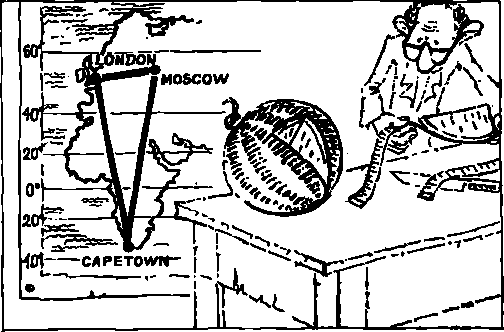
\includegraphics[width=0.8\textwidth]{figures/fig-07-02.pdf}
\caption{The Pythagorean theorem is not valid on the surface of the earth.}
\label{fig-7.2}
\end{figure}

If you want to, I can show you that the Pythagorean theorem has failed. Take a map of important airlines (\figr{fig-7.2}) and take the triangle Moscow-Capetown- London. On the map it turns out to be an almost exact right triangle and so the sum of the squares on the sides must be equal to the square on the hypotenuse. Well, you can guess again. Let’s figure it out exactly: the distance from Moscow to London is \SI{2490}{\kilo\meter}, from Mos­cow to Capetown it is \SI{10130}{\kilo\meter}, and from London to Capetown \SI{9660}{\kilo\meter}. The theorem fails completely. Our geometry does not hold true at all on a map. The laws of geometry in a plane depicting the globe differ from ``or­dinary'' laws.

Take a look at the map of the hemispheres and you will see it has ``edges''. But this is an illusion. Actually, if one moves over the surface of the earth, he never comes to any ``edge of the earth''.

There is even a joke to the effect that Einstein’s son asked his father why he was so famous. Said the great Einstein: ``I was lucky, I was the first to notice that a bug crawling on the globe can crawl around the equator and come back to the starting point.'' That observation does not represent a discovery of course. But extend it to the three-dimensional space of the universe; maintain that the universe is finite and closed like a two-dimen­sional surface bounding the globe (thus laws of ``ordinary'' geometry do not hold true any longer); then from that draw the conclusion that all points of the universe are of an equal status in the same sense that all points on the surface of the globe are -- well, all that requires ex­ceptional intellectual courage.

Now we can conclude that if we earthlings observe that all galaxies are racing away from us in all directions, then an inhabitant of the planet of any star will observe the same; he will arrive at the same conclusions concerning the nature of motion of the stellar world and will measure the same velocities of the galaxies as the earth dweller.

The model of the universe advanced by Einstein in 1917 was a natural consequence of his so-called general theory of relativity (that part of the theory that we discussed in \hlgray{Chapter \ref{ch-04}} is called the special theory of relativity).

However, Einstein did not envisage the possible expanding of a closed universe. The fact that a closed universe must expand was demonstrated in 1922-1924 by the Soviet scientist Alexander A. Friedman (1888-1925). It turned out that the theory requires that the universe either ex­pand or have alternating expansions and contractions. At any rate it cannot be static. We can accept either one of these two viewpoints, that is, we can assume that we are now living in an epoch of expansion of the universe, or we can assume that the universe was a ``cosmic egg'' some time ago (calculations show this time lapse to be equal to several tens of thousands of millions of years) and that it exploded and the debris has since been ex­panding.

It is important to have a clear understanding that the idea of an initial explosion is in no way connected with the concept of a creation of the world. It may very well be that attempts to look too far into the future and too far into the past and also out to excessively great distances are unjustified within the framework of existing theories.

Let us take a simple example and examine it in the light of a scheme that appears today to be quite reason­ able. We measure the red shift of the spectral lines of radiation coming to us from distant galaxies. Using the Doppler equation, we estimate the velocities of the stars. The farther they are away from u the faster they appear to be moving. Telescopes report speeds of recession of still more distant galaxies: ten thousand kilometres a second, a hundred thousand kilometres a second, and faster still. Now, there must be a limit to these recessional speeds. The point is that if a galaxy is moving away from us with the velocity of light, we will in principle never be able to see it, and all because, according to the Doppler equation, the frequency of light will vanish (become zero). No light would ever reach us from such a galaxy.

What are the greatest distances we are capable of mea­suring with the very best of the excellent instruments at our disposal? Our estimate will of course be extremely approximate. At any rate, we should not complain about not being able to look far enough away: the distances we are talking about run into thousands of millions of light years!

To speak of still greater distances is clearly meaning­ less. We might put it thus: within the framework of existing ideas, to talk about distances exceeding thousands of millions of light years is physically meaningless for the simple reason that no method has been devised for measur­ing such distances.

The situation here is much like that concerning the trajectory of an electron: it cannot be measured for the simple reason that the very concept is meaningless.

\section{The General Theory of Relativity}

The special theory of relativity made it necessary to introduce corrections into the laws of mechanics of bodies moving with velocities close to the velocity of light. The \emph{general theory of relativity} introduces corrections into cus­tomary concepts concerning space when we deal with great distances. It is precisely for this reason that a discussion of the general theory is fitting in a chapter devoted to the physics of the universe.

The general theory of relativity rests on the following principle: there are no experiments capable of distin­guishing the motion of bodies under the action of a grav­itational field from the motion of such bodies in an appropriately chosen noninertial reference frame.

Let us consider a few simple examples. We are in a lift falling with acceleration $a$. Stretch out your hand and drop a ball. How will it fall? As soon as it is released, it will begin (according to the viewpoint of the inertial observer) its free fall with acceleration $g$. Since the lift is falling with acceleration $a$, the acceleration with re­spect to the floor of the lift will be $(g-a)$. An observer in the lift can describe the motion of the falling body with the help of the acceleration $g'=g-a$. In other words, an observer in the lift need not speak of any acceleration of the lift by ``changing'' the acceleration of the field of gravity in his frame of reference.

Now let us compare two lifts. One hangs motionless above the earth, the other is in motion in interplanetary space with acceleration a with respect to the stars. All bodies in the lift that is stationary above the earth can fall freely with acceleration $g$. And so can bodies inside the interplanetary lift. They will ``fall'', with acceleration $-a$, to the ``bottom'' of the lift. Here, the bottom will be the wall opposite the direction of acceleration.

It turns out that the action of a gravitational field and manifestations of accelerated motion are indistin­guishable.

The behaviour of a body in a reference frame under­ going accelerated motion is the same as the behaviour of a body in the presence of an equivalent gravitational field. However, this equivalence can be complete if we confine ourselves to observations over small portions of space. Indeed, imagine a ``lift'' with a floor measuring thousands of kilometres. If such a lift hangs motionless above the earth, the phenomena taking place in it will be different than in the case where the lift is moving with acceleration a relative to the fixed stars. This is clear from \figr{fig-7.3}: in one case the bodies fall at an angle to the bottom of the lift, in the other case they fall verti­cally.

\begin{figure}[!ht]
\centering
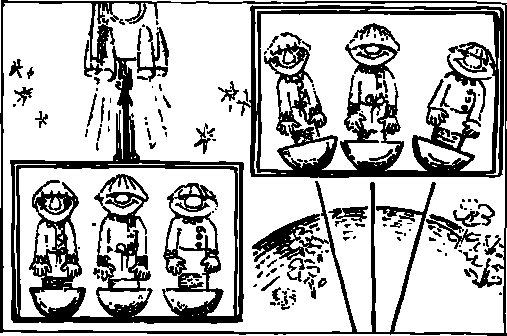
\includegraphics[width=0.8\textwidth]{figures/fig-07-03.pdf}
\caption{The equivalence principle.}
\label{fig-7.3}
\end{figure}

Thus, to summarize, the principle of equivalence holds true for portions of space in which the field may be re­garded as uniform.

The principle of equivalence of a gravitational field and a properly chosen local reference frame leads us to an important conclusion: a gravitational field is linked up with the curvature of space and a distortion in the flow of time.

Two observers are engaged in measuring distances and time intervals. They are interested in events occurring on a rotating disk. One observer is located on the disk, the other is motionless (relative to the stars). Incidentally, only the researcher on the disk is working. The fixed observer merely watches the work of his colleague.

The first experiment consists in measuring the radial distance, that is, the distance between two objects located on the same radius of the disk at different distances from the centre. The measurements are performed in the ordi­nary way: a standard ruler is laid off between the ends of the segment of interest. From the viewpoint of both in­vestigators, the length of the ruler laid perpendicularly to the direction of motion is the same. And so there will be no argument between the two observers as to the length of the radial line-segment.

Now the disk dweller initiates his second experiment. He would like to measure the length of the circle. The ruler must now be laid down along the direction of mo­tion, and of course we have to take into account the curvature of the circle. We therefore use a small ruler so that we can equate the length of a tangential line-segment with the length of the arc. The observers will not argue about the number of times the ruler fitted into the length of the circumference of the circle. And never­theless their opinions about the length of the circum­ference will differ. The point is that the fixed observer will claim that the ruler contracted because, in the second experiment, it lay along the direction of motion.

And so the radius of the circle is the same for both observers but the length of the circumference of the circle is different. The fixed observer concludes that the formula for the length of the circumference of a circle, $2\pi r$, is incorrect. He says that the length of the circumference is greater than $2 \pi r$.

This example shows us how the theory of relativity comes to a rejection of Euclidean geometry or (what is the same thing only said in different words) to the concept of curved space.

Similar ``madness'' is seen in the clock experiment.


Clocks fixed at different distances from the axis of rota­tion have different rates, and they are all slower than the fixed clock. Also, the farther a clock is from the centre of the disk the slower it goes. A fixed observer would say that you can use clocks and rulers on the disk only if you are located at a definite distance from the centre. Space and time possess local peculiarities.

Now let us recall the equivalence principle. Since local peculiarities of time and space manifest themselves on a rotating disk, this means that phenomena in a gravita­tional field behave in the same manner. The situation on the disk is the same as in the lift depicted in \figr{fig-7.3}. Accelerated motion is indistinguishable from gravitation acting against acceleration (in the direction opposite ac­celeration).

What this means is that a local curvature of space and time is equivalent to the presence of a gravitational field.

The closed nature of the universe that we discussed in the preceding section can undoubtedly be regarded as corroborating the general theory of relativity.

By applying rigorous mathematical reasoning, it is possible to derive a number of quantitative corollaries from the intricate equations of the general theory of relativity. First, Einstein demonstrated that a ray of light passing close to the sun must be deflected. The deflection of a ray of light passing very close to the sun should amount to 1.75 seconds of arc. Actual measure­ments yielded a figure of 1.70. Second, the orbit of the planet Mercury (the perihelion of the orbit, to be precise) should turn in its plane. Calculations show that in one century this should amount to 43 seconds of arc. Experi­ment has revealed precisely that number. And now a third prediction that was confirmed by experiment: a photon used up energy (and hence the frequency of the light changes) in overcoming gravitational forces.

The general theory of relativity is one of the greatest attainments of human thought. It has played a tremen­dous role in the development of our ideas about the universe and has revolutionized physics.

\section{Stars of All Ages}

The physics of the universe is still growing fast, it cannot at all be regarded as a fully developed science like, say, the mechanics of low velocities or thermodynamics. There is therefore every reason to believe that stellar investigations will lead to discoveries of new laws of nature. So far this has not occurred, but the picture of the universe drawn from time to time by the popularizing physicist is constantly changing. What I have to say here and now will, in a decade or so, most likely undergo considerable change.

Astronomers have long realized that there are different kinds of stars. With the help of the telescope, the spec­trograph, and the interferometer we can determine many physical quantities that go to classify the stars.

As may be expected by analogy with terrestrial experi­ments (see page \pageref{bbr-ref}), the maximum intensity of the spec­trum defines the surface temperature of a star. The ob­served colour of the star is uniquely related to this tempera­ture. If the temperature is from 3 to 4 thousand degrees, the colour is reddish, if the temperature is between 6 and 7 thousand degrees, the star is yellowish. Pale blue stars have temperatures exceeding 10-12 thousand degrees. When physicists were able to get out into space, they found stars whose maximum radiation lies in the region of $X$ rays and gamma rays. This means that the tempera­tures of such stars can reach into millions of degrees.

Another important characteristic of a star is the total energy of the spectrum that reaches us. This is the \emph{lumi­nosity} of the star. The colossal differences in luminosity may be connected with the size of the star, its distance from us, and its temperature.

As to chemical composition, stars consist largely of hy­drogen-helium plasma. Our sun is a rather typical star. Its chemical composition has been determined more or less precisely from the type of spectrum and from theoretical calculations of the energy of its radiation. Hydrogen makes up 82\% and helium 18\%. All other elements come to only 0.1\% of the total mass of the sun.

The atmospheres of many stars exhibit powerful mag­netic fields that are thousands of times stronger than the magnetic field of the earth. We know about this due to spectral analysis, since the spectral lines split in magnetic fields.

The interstellar medium is rarefied to an extent beyond all imagination: one cubic centimetre of outer space con­tains one atom. This is a good time to recall that one cubic centimetre of the air we breathe contains \num{2.7d19} molecules, on the average. There are regions of space where the density of the interstellar gas is appreciably higher than the average. Besides gas we encounter dust, which consists of particles of size \num{d-4} to \SI{d-5}{\centi\meter}.

It can be assumed that stars are formed out of this gaseous-dust medium. Under the influence of gravitation­ al forces, a cloud begins to contract into a sphere. In the course of hundreds of thousands of years it contracts and the temperature of the star increases making it visible in the heavens. Of course, the time required for this depends on the size and, hence, the mass of the con­densing cloud.

As the contraction continues, the temperature in the interior of the star rises and attains a value at which a thermonuclear (fusion) reaction can start up. Four nuc­lei of the hydrogen atom combine into a single nucleus of a helium atom. Recall that in the process, 4.0339 atomic mass units of four hydrogen atoms are converted into 4.0038 atomic mass units of the helium atom. Thus a mass equal to 0.0301 unit is converted into energy.

The burning of hydrogen that takes place in the deep interior of a star can continue for different time intervals depending on the mass of the star. For the sun, this time interval is equal to between 10 and 20 thousand million years. That is the stable-state period of the star. The forces of gravitational attraction are balanced by the internal pressure of the hot nuclei that tend to blow up the star. A star is hence something like a gas cylinder. The walls of the cylinder, so to speak, are the gravita­tional forces.

When the supply of hydrogen fuel comes to an end, the internal pressure diminishes, and the core of the star begins to collapse.

What happens next? To that question the theoretician replies that everything depends on whether the star is able to shrug off its outer shell. If the star does throw off the outer shell, the mass of the star becomes roughly half that of the sun, and then forces take over that are capable of counteracting the gravitational forces. The result is a tiny star with a high surface temperature. It goes by the name of \emph{white dwarf}.

What next? Again the fate of the star depends on the mass. If the white dwarf has a mass less than one and a half solar masses, then it will die out slowly with no dramatic events taking place. The radius will diminish and the temperature will fall. Ultimately, the dwarf will turn into a cool star the size of the earth. Such is the demise of most stars.

Now if the mass of the white dwarf that took shape after the star with fuel expended has thrown off its outer shell is more than one and a half solar masses, then contraction does not come to a halt at the white-dwarf stage. Electrons merge with protons to form a \emph{neutron star}, which measures only a few tens of kilometres across.

Calculations show that a neutron star should have a temperature of the order about ten million degrees. It has a maximum radiation in the region of $X$ rays.

We have just discussed the history of a star that is able to throw off the outer shell. However, the mathemat­ical equations do not insist on such disrobing. Now if a celestial body retains the mass of, say, ten of our suns, then the gravitational attraction would simply destroy the star. Where the star once was there would be a \emph{black hole}.

At what stage in the compression process should this take place, and what does the term ``black hole'' stand for?

Let us recall the simple laws that underlie the launching of space craft from the earth (see the first book in this series). To escape from the earth's gravitational pull requires a velocity of 11 kilometres per second. This velocity is given by the equation
\begin{equation*}%
v^{2} = \gamma \frac{M}{R}
\end{equation*}
From this equation it is evident that as a sphere of definite mass contracts, the escape velocity of a rocket from such a body into outer space will be constantly increasing. But the limiting velocity is equal to 300 000 kilometres per second! If a stellar sphere of given mass contracts to a ball having radius
\begin{equation*}%
R = \gamma \frac{M}{(\SI{300000}{\metre\per\second})^{2}}
\end{equation*}
then it becomes impossible to escape. In other words, anything at all can go into what was once a star (say, a ray of light or other electromagnetic radiation), but it cannot go out; it cannot escape from the hole. Black hole is indeed a very appropriate designation. Using the above equation, we can see at once that black holes with from 3 to 50 solar masses will be from 60 to 1000 kilo­metres across.

A few words are now in order about how to search for black holes. The reader may think that this problem is too small for a little book devoted to the whole of physics, but I think the very method of approaching such a search is highly instructive. The talent of a scientist is revealed precisely in the search for indirect proofs of a model whose properties cannot be demonstrated directly.

At first glance, the problem does indeed appear to be exceedingly complicated, if not downright unsolvable. A black spot in the sky 1000 kilometres across corresponds to a millionth of one second of arc. No telescope could detect a black hole.

Over twenty years ago the Soviet physicist Ya. Zeldovich proposed a search for black holes based on the idea that their presence in the sky should affect the be­haviour of nearby visible bodies. Together with his coworkers, he conducted a systematic examination of star catalogues in order to find a visible star that might be revolving about a black hole. Such a star would appear to be alone but its revolution would indicate that the spectral lines would periodically be displaced redwards or bluewards depending on whether the star was moving away from us or towards us.

Research workers in other countries also entered the search and a certain number of suitable stars were found. From the amount of the Doppler shift we can give a rough estimate of the mass of the star about which the visible satellite star is revolving. Some invisible can­didates were selected with masses three times the solar mass. Thus, these could not be white dwarfs or neutron stars.

And yet all of this is not enough to claim that such an exotic entity as a black hole does indeed exist. Any opponent could advance a whole series of explanations for the periodic Doppler shift.

However, there is one phenomenon that we can call to our aid. A black hole is capable of drawing into itself gas from its satellite star. As this gas falls into the black hole, it should heat up intensely and should emit $X$ rays. True, neutron stars and white dwarfs are also capable of drawing in gas, but such stars, as we have already pointed out, can be distinguished from a black hole by their mass.

Just recently a star was found that satisfied all re­quirements for the satellite of a black hole. New experi­ments will undoubtedly follow and also detailed theoret­ical calculations whose aim is to predict the peculiari­ties of the $X$-ray spectrum emanating from the surround­ ing space of a black hole. The near future will surely show us how often these amazing ``bodies'' turn up in the universe. There are grounds to believe that there may be large black holes and mini-holes of mass of the order of \SI{d-16}{\gram}. Such holes less than an atomic nu­cleus in size may suddenly die out and in their final act return the energy contained in them. This energy would be so great as to satisfy all terrestrial needs for many years! What a marvelous topic for science fiction writers.

\section{Radio Astronomy}
The photograph shown in \figr{fig-7.4} depicts a parabol­ic radio antenna that focuses incident parallel radio beams. The beams come to a point and enter a special receiver. The signal is then amplified by electronic equip­ment. The parabolic antenna shown in the figure is that of the Effelsberg Radio Observatory (near Bonn, West Germany). This fully steerable radio telescope (about 100 metres in diameter) is used in joint research by teams of scientists from many countries, including the USSR.

\begin{figure}[!ht]
\centering
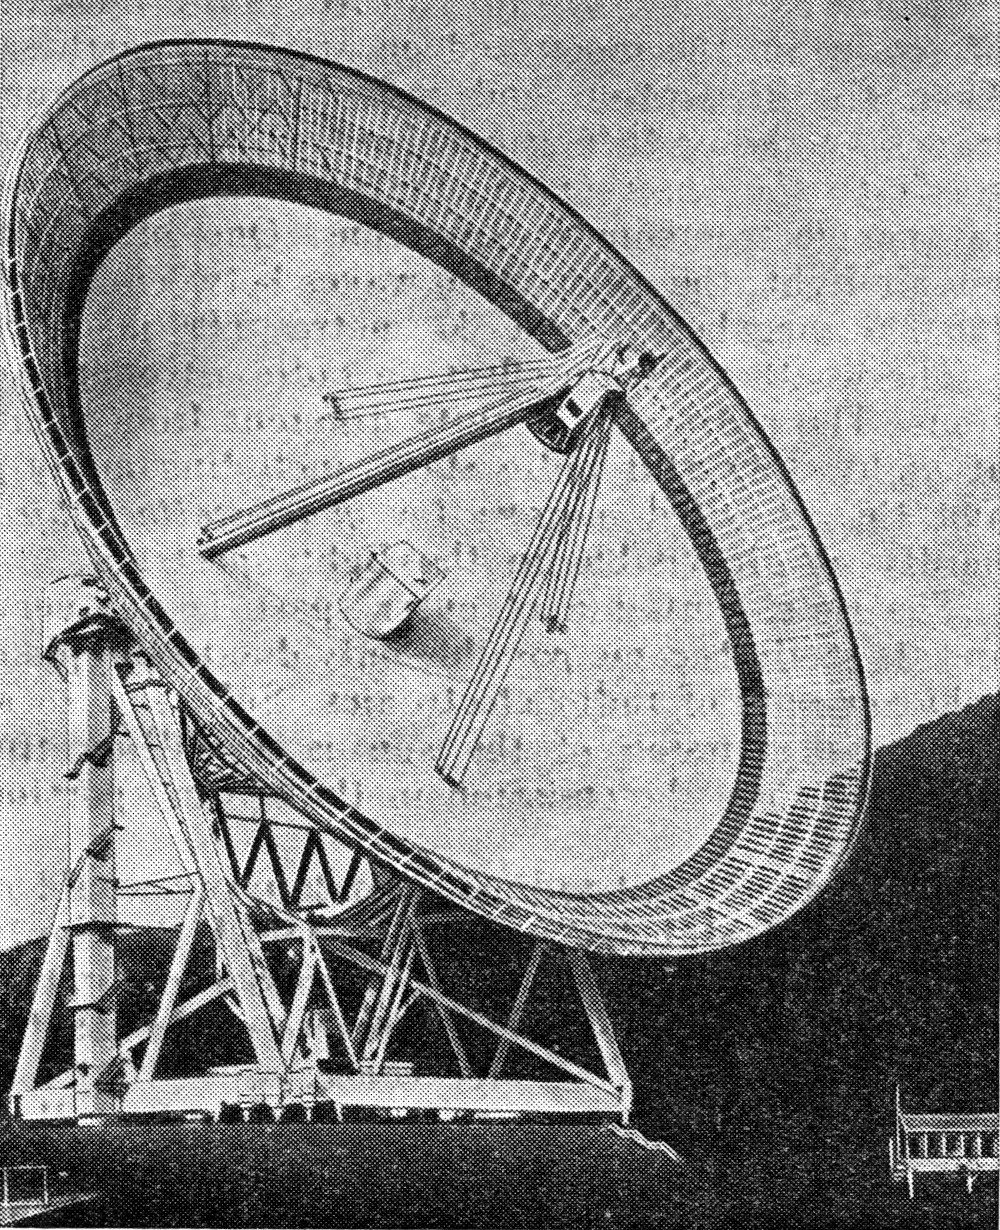
\includegraphics[width=0.8\textwidth]{figures/fig-07-04.jpg}
\caption{The radio telescope of the Effelsberg Radio Observatory.}
\label{fig-7.4}
\end{figure}


Such telescopes are extremely sensitive. They can be steered in any direction and the antenna is capable of detecting energy fluxes of the order of \SI{d-28}{\watt\second\per\metre\squared}. Fantastic!

Radio astronomy has led to fundamental discoveries in the physics of the universe.

In the not too distant future radio telescopes will be set up on the moon and on artificial earth satellites. Then the absorption and reflection of electromagnetic waves by the earth’s atmosphere will cease to be an ob­stacle to the observer. So far there are two ``windows'' in the electromagnetic spectrum. One of them lets in visible light, the other radio waves between 2 centimetres (15000 megahertz) and 30 metres (10 megahertz).

The weather has no effect on radio-astronomy observa­tions. The radio sky is quite different from what we see at night. Powerful radio stars, including many galaxies and the so-called \emph{quasars} (or \emph{quasi-stellar objects}), are hardly at all visible in the light spectrum.

The radio emission of outer space is not very strong and its study became possible only due to the phenomenal achievements of radio electronics. Suffice it to say that the radio emission of the sun is a million times less powerful than the emission in the optical portion of the spectrum.

And yet, without radio spectroscopy we would not have been able to establish many important facts. For instance, a big role in understanding processes occurring in the universe is played by measurements of the residual emis­sion of explosions of \emph{supernovae}.

Neutral hydrogen emits a strong wave of 21 centime­tres. Measurements of the intensity of this radio emission have enabled scientists to sketch a pattern of the distri­bution of interstellar gas in space and follow the move­ments of gaseous clouds.

A large number of radio galaxies and quasars have been found at distances extending to the very limit of obser­vational capabilities. Suffice it to say that the red shift in the radiation coming from these sources reaches a value of 3.5. The \emph{red shift} is defined as the ratio of the difference between the emitted and received wavelength to the magnitude of the emitted wavelength. This means the difference is 3.5 times greater than the wavelength of the radiation.

Radio methods have enabled us to look out to the very fringes of the universe. Radio-astronomy investigations have enabled us to clarify the nature of the cosmic radiation that comes to us from the outer reaches of the universe.

\section{Cosmic Rays}

Studies that are now conveniently conducted in outer space beyond the earth’s atmosphere demonstrate that our planet is under a constant bombardment by streams of nuclear particles moving at velocities close to the velocity of light itself. These particles have energies be­ tween $10^{8}$ and \SI{d20}{\electronvolt}. An energy of the order of \SI{d20}{\electronvolt} is eight orders of magnitude greater than the energy of the most powerful particle accelerators we have been able to build.

The primary cosmic radiation consists mainly of protons (about 90\%); the remainder is made up of heavier nuclei. Naturally, when cosmic-ray particles collide with molecules, atoms, and nuclei, they can make elementary particles of all types. But astrophysicists are particularly interested in the primary radiation. How are such ener­getic particle fluxes created? Where are the sources of cosmic rays located?

A long time ago it was demonstrated that the sun is not the main source of cosmic radiation. But if that is so, then the responsibility for generating cosmic rays cannot be shifted to other stars either, for they are in no way different (in principle) from our sun. Then who is to blame?

In our Galaxy we have what is known as the Crab Nebula that was formed in the explosion of a star in the year 1054 (don’t forget that the sky has been under observation for many thousands of years). This has been shown to be a source of radio waves and cosmic radia­tion -- a coincidence that resolves the mystery of the tre­mendous energies of cosmic protons. As we know, a par­ticle can build up energy by spiralling about a magnetic line of force. All we need to do is presume that the elec­tromagnetic field generated in the explosion of the star plays the role of a synchrotron, and then the enormous energy acquired by a particle as it journeys along a spiral curve about a line of force over periods of thousands of years can reach truly fantastic figures (like those we have mentioned).

Calculations show that after covering a distance equal to the diameter of our Galaxy, a cosmic particle cannot acquire more energy than \SI{d19}{\electronvolt}. Apparently, particles of maximum energy come to us from other galaxies.

Naturally we need not assume that only stellar explo­sions generate cosmic radiation. Any sources of radio waves can also be sources of cosmic radiation.

Cosmic rays were discovered at the start of this century. Electroscopes carried aloft in balloons revealed some exciting facts. Researchers found that the discharge of an electroscope at high altitudes proceeds much more quick­ly than it does at sea level.

It became clear that the usual falling of the leaves of the electroscope is not the result of imperfections in the instrument, but a phenomenon due to the action of some kind of external factors.

In the 1920s, physicists were quite convinced that the ionization of the air that removes the charge from an electroscope is undoubtedly of extraterrestrial origin. The American physicist Robert Andrews Millikan (1868-1953) was the first to state this confidently and he gave the phenomenon its modern name: \emph{cosmic rays} (or \emph{cosmic radiation}).

In 1927, the Soviet scientist D. V. Skobeltsyn obtained the first photograph of the tracks of cosmic rays in an ionization chamber.

The energies of cosmic particles were determined by methods that we have already described elsewhere. They turned out to be tremendous.

In their studies of cosmic rays, physicists have made a number of very remarkable discoveries. For one thing, the existence of the positron was demonstrated in precisely this way. The same goes for \emph{mesons}, which are parti­cles with mass intermediate between the mass of the proton and that of the electron; they too were first detected in cosmic radiation.

Studying cosmic rays continues to be one of the most exciting fields of physical investigation.

\begin{center}
\pgfornament[width = 2cm,
             color = black!70]{80}
\end{center}


The very incompleteness of astrophysics makes it dif­ficult to describe it in a single chapter of a small book devoted to merely an introduction of the reader to the basic facts and ideas of physics at large. I could only choose a few of the many physical problems that deal with the universe, only those that I consider to be of special interest.